\chapter{Concepts}
\label{chap:concepts}

\section{User Interface}

\begin{figure}
	\caption{\label{fig:firstmockup}A first overview of the screen space distribution}
	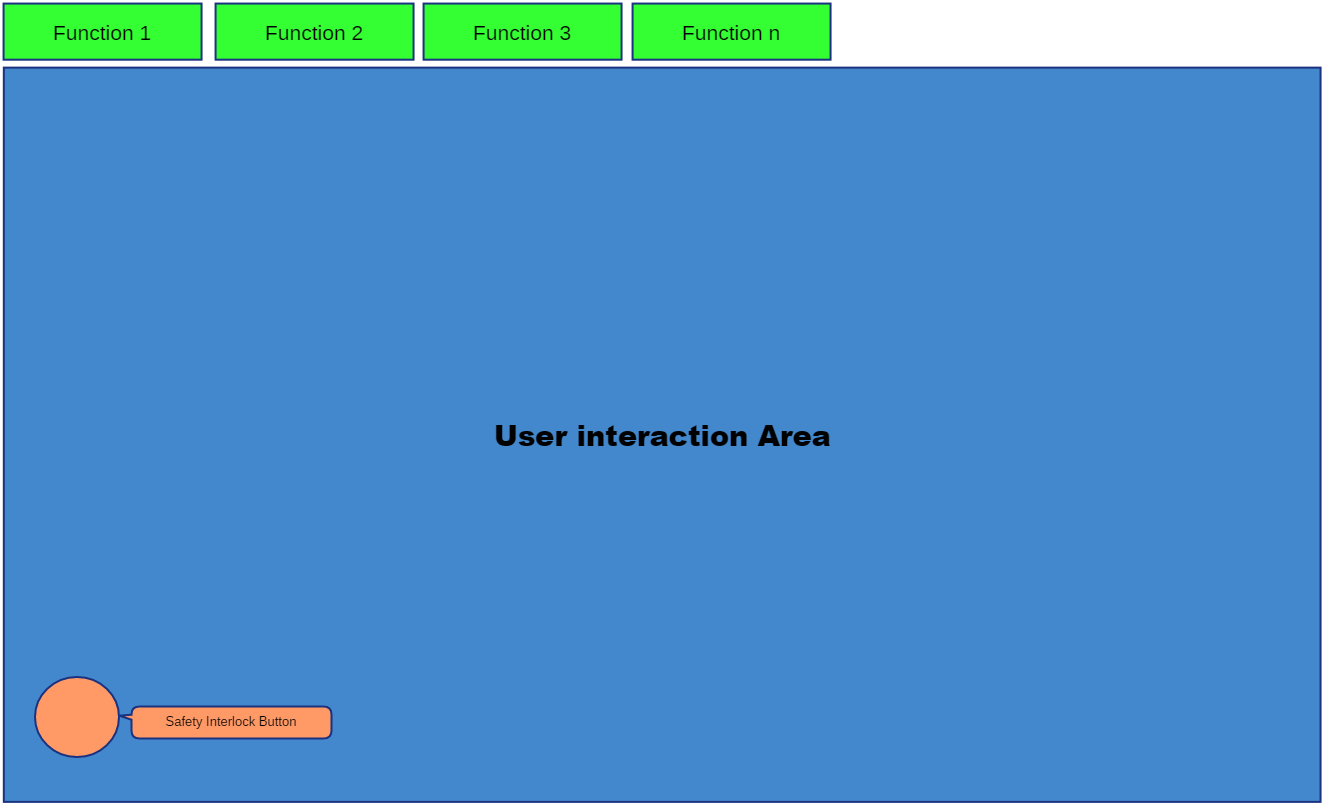
\includegraphics[width=0.9\textwidth]{assets/chpt_concepts/main_touch_interface.png}
\end{figure}

\subsection{Desired position of the Android Tablet}
The application (and thus the screens within it) will be designed for the tablet to be placed in front of the operating person on a table. The person should have clear sight on the controlled robot. It seems sensible to place the tablet on the table in front of the robot while looking at it. Most interactions with the application will be performed by touch gestures using the right hand. For better usability a housing or case can be used to position the tablet at a slight angle to the table. 
% TODO FOTO VOM TABLET AUF TISCH

Interaction with the application is done using the commonly known touch gestures like
\begin{itemize}
	\item Touch (short press on the screen)
	\item Long press (finger remains on a control for a longer period of time)
	\item 1-Finger-Movement
	\item 2-Fingered gestures (\textit{Pinch-Zoom}, Rotation)
	\item 3-Fingered gestures (Rotation, Movement)
\end{itemize}

\subsection{General Screen Layout}

As a screen of a diagonal size of 10 inches (25.4cm) is very limited compared to the size of the robot's workspace good considerations have to made according to a well-designed user interface. Since we are mainly operating the robot with touch gestures, significant parts of the screen should be blank, as only few information can be displayed while the user poses his hands above or on the screen. Figure \ref{fig:firstmockup} gives a first overview of how the portions of the screen shall be distributed. The biggest part of the screen is reserved for touch interactions by the user. Since multiple approaches to control the robot shall be implemented, the method shall be selected and switched using a tabbed layout with the tabs on the top, as they then use the least space of the screen.

\subsubsection{Interlock Button}
On all screens where the robot can be remotely operated, a security interlock button shall be displayed. For the actions on the screen to have effect on the robot (i.e. to be sent to the controller) the button shall remain pressed. This implements the functionality of a dead-man-switch, stopping all robot action once released. Although this is only a software measure it should be a good solution against unwanted movements of the robot as the button can easily be released when pressed with a single finger of the left hand. \textbf{Of course, this software measure does not replace hardware safety measures like emergency switches, but only supports them.}

\subsection{Grasp Synergy Screens}

\begin{wrapfigure}[12]{l}{0.6\textwidth}
	\caption{\label{fig:screen:synergy}Synergy control screen}
	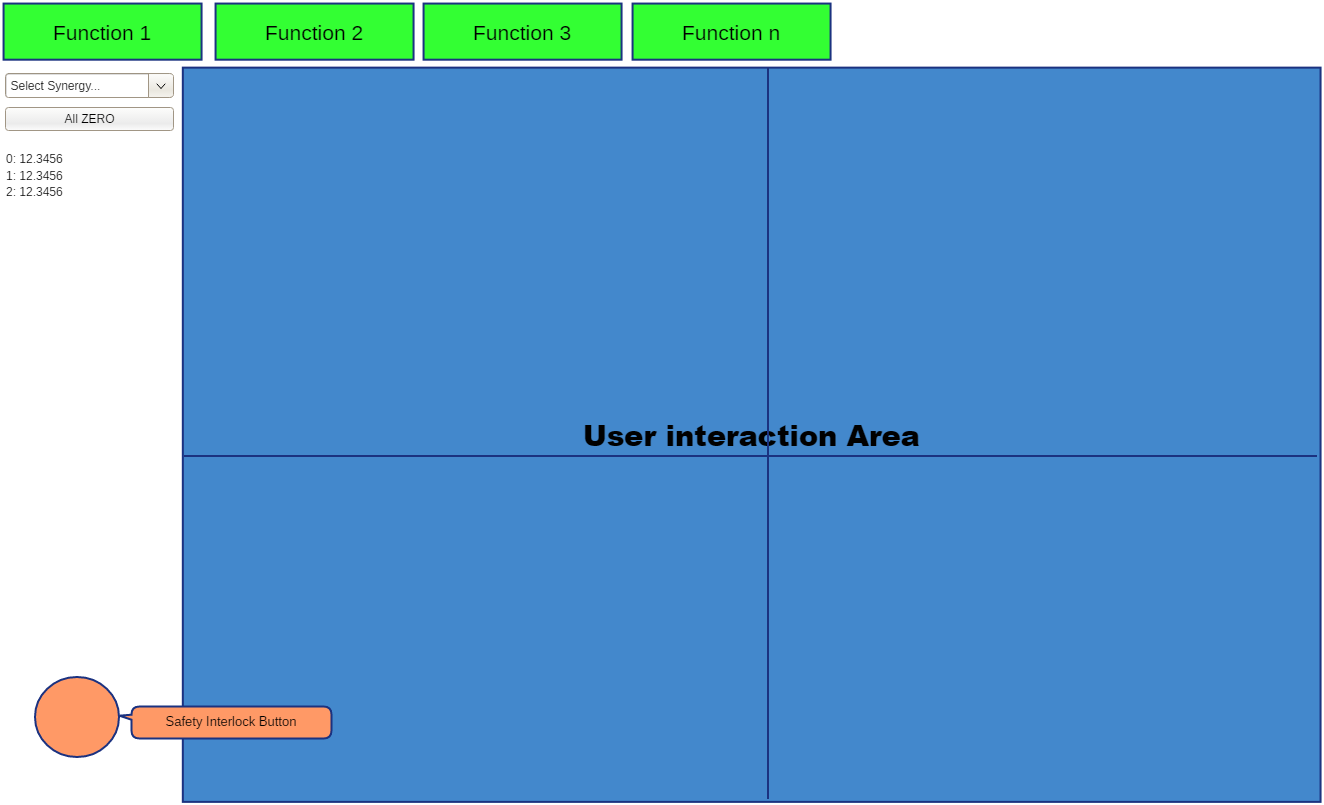
\includegraphics[width=0.6\textwidth]{assets/chpt_concepts/grasp_synergy_page}
\end{wrapfigure}

As the control of grasp synergies allows multiple different types of synergies to be selected, a drop-down selection of the synergy shall be displayed to the left side of the screen. This keeps the right side of the screen clear for better operability by right-hand users. Additionally, a cross of lines shall be displayed on the screen so the user knows where the middle of the touch interaction area is. As described later, this is particularly important in the approach with absolute synergy control (See Chapter \ref{sec:synergies:absolute}). To give the user some information about the state of a synergy, the values of significant amplitudes applied to the synergy shall also be displayed on the left hand side of the screen. A button to set the hand into the synergy's idle state (i.e. all significant amplitudes set to $0$) is also sensible to be implemented. A sample of how this screen could look like is demonstrated in Figure \ref{fig:screen:synergy}.

\subsection{Direct Fingertip Mapping Screen}

As there are no additional controls required to control the direct fingertip mapping, the control screen looks mostly like the general touch interaction screen seen in Figure \ref{fig:firstmockup}.

\subsection{Single Axis/Joint Control}

\begin{wrapfigure}[11]{r}{0.4\textwidth}
	\caption{\label{fig:axiscontrol}Axis control widget with different status indicators}
	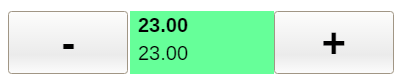
\includegraphics[width=0.4\textwidth]{assets/chpt_concepts/AxisControlGreen}
	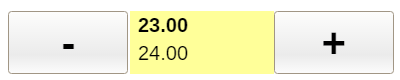
\includegraphics[width=0.4\textwidth]{assets/chpt_concepts/AxisControlYellow}
	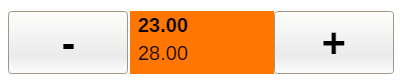
\includegraphics[width=0.4\textwidth]{assets/chpt_concepts/AxisControlRed}
\end{wrapfigure}

An interface shall be implemented to give users the ability to control each joint of the robot individually. This is sensible for a variety of reasons. Firstly, it might sometimes be required to move the robot out of a specific state by moving just one axis and not by applying multiple changes at once. Possible scenarios for this use case could be a state where the robot could harm users or the environment if uncontrolled or unpredictable movements occur. An interface to control joints individually is also very practical for testing purposes, for example if one part of the robot is suspected to be broken.

Within this interface, the currently measured joint angle shall be displayed for each joint, next to the currently set target value (printed in bold). This gives the user a good insight of what state the robot should be in according to the program and what state it is actually in. This shall be supported by a coloured indicator, giving a quick visual feedback on the difference of the target and actual joint angles $\Delta \alpha = |\alpha_{actual} - \alpha_{target}|$. The colours of the visual feedback shall be:

\begin{itemize}
	\item Green for $\Delta\alpha \leq 0.5^\circ$
	\item Yellow for $0.5^\circ < \Delta\alpha \leq 2.5^\circ$
	\item Red for $\Delta\alpha > 2.5^\circ$ 
\end{itemize}

The buttons to move the axis shall be displayed right and left of the angle displays. The visual feedback shall be shown as the background of the angle values. All these requirements put together, an axis control widget for a single joint or axis could look like depicted in Figure \ref{fig:axiscontrol}. To each control widget, a heading will be added to unambiguously denote which axis or joint will be controlled when using the corresponding buttons.

Multiple of these widgets shall be added to the axis control screen, one for each controllable joint or axis. This will result in a screen containing 29 of these (22 for the hand, 7 for the robot arm). To get an idea of how the control screen for individual joint control will look like, refer to Figure \ref{fig:axiscontrol:screen}\footnote{Please note, however, that the number of hinted joint control widgets does not resemble the actual number of controllable joints for each part of the robot.}. 

\begin{figure}
	\caption{\label{fig:axiscontrol:screen}Axis control screen draft}
	\frame{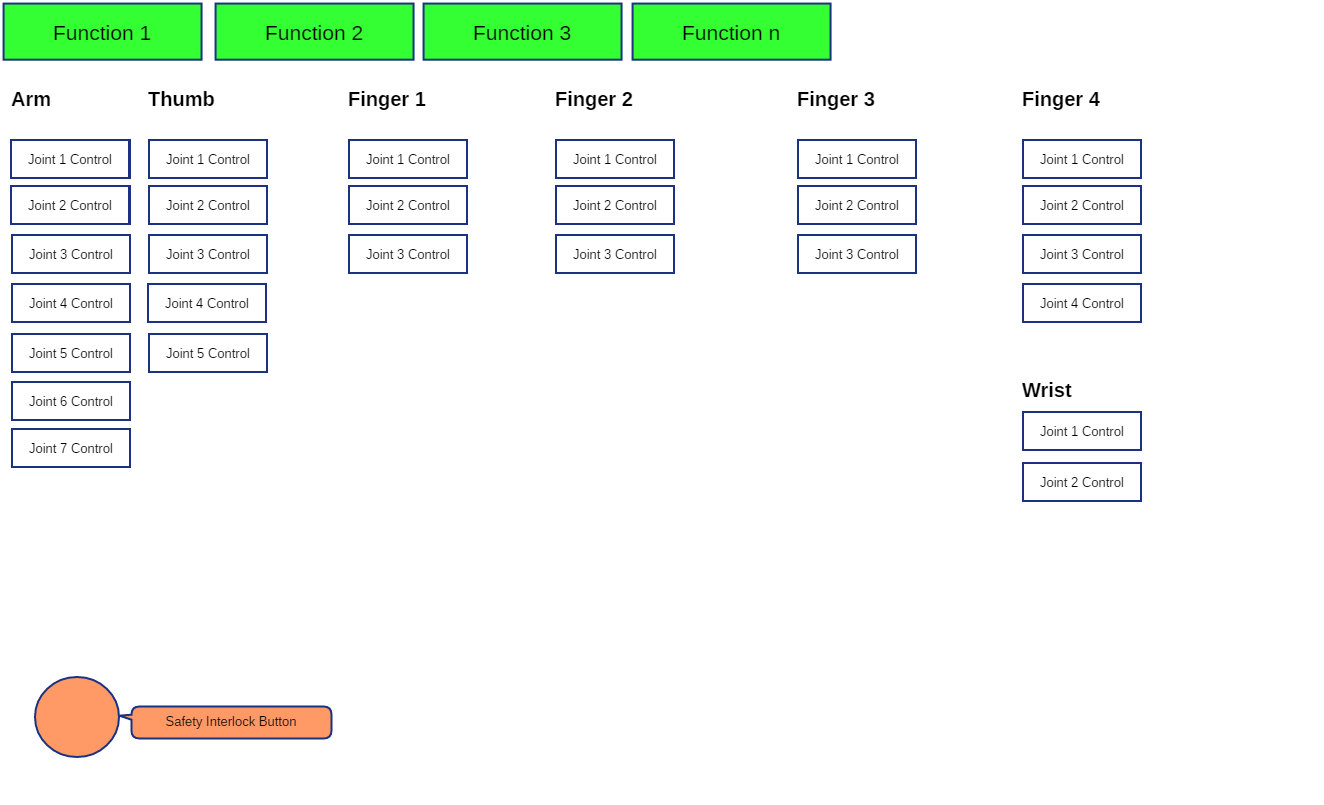
\includegraphics[width=0.8\textwidth]{assets/chpt_concepts/AxisControlPage}}
\end{figure}

\section{Using the BioIK Service}
\label{sec:robotarm:ctrl}

The BioIK serivce (see Section \ref{sec:bioik}) is used according to the description in Section \ref{sec:using_services}. The important messages types are:
\begin{itemize}
	\item \textbf{GetIK} The combined Request/Response service message type
	\item \textbf{GetIKRequest} The message type containing the request to the service
	\item \textbf{GetIKResponse} The message type containing the response of the service
	\item \textbf{IKRequest} The actual request data
	\item \textbf{IKResponse} The actual response data
\end{itemize}

In the process of getting joint data from the BioIK service, the message types \textit{IKRequest} and \textit{IKResponse} are most important, as they contain the data needed on both sides. As the used message types contain a large number of members, only those significant for this thesis will be discussed within this section.

\begin{table}
	\caption{Important contents of the IKRequest message type\label{tab:msg:ikrequest}}
	\begin{tabularx}{\linewidth}{|l|X|}
		\hline
		\textbf{Field} & \textbf{Description} \\
		\hline
		string group\_name & The MoveGroup name of the robot. Fixed to \textit{lwr\_with\_c5hand} here \\
		\hline
		bool approximate & If true, an approximate solution is returned when no exact solution could be found by the IK solver \\
		\hline
		duration timeout & The timeout after which the solver stops looking for solutions. If no solution was found by then, an approximate solution is returned if approximate is true, otherwise no solution is returned. Fixed to one second here. \\
		\hline
		int32 attempts & Number of attempts the solver shall take. Fixed to 1 here. \\
		\hline
		string[] fixed\_joints & Names of the joints the IK solver shall not move while looking for solutions. \\
		\hline
		bool avoid\_collisions & If true, the BioIK solver tries to find solutions that to not collide with the environment (and the robot itself). \\
		\hline
		RobotState robot\_state & The current state of the robot. Contains a JointState message containing the current joint angles of all joints. These values are taken as a starting point while searching for solutions. \\
		\hline
		PositionGoal[] position\_goals & The positions of multiple end-effectors that shall be reached with the IK solution. \\
		\hline
		PoseGoal[] pose\_goals & The poses of multiple end-effectors that shall be reached with the IK solution. A pose goal is similar to a position goal, but extends it by a desired orientation. \\
		\hline
		OrientationGoal orientation\_goals & The orientations multiple end-effectors shall have within the IK solution. \\
		\hline
	\end{tabularx}
\end{table}

\begin{table}
	\caption{Important contents of the IKResponse message type\label{tab:msg:ikresponse}}
	\begin{tabularx}{\linewidth}{|l|X|}
		\hline
		\textbf{field} & \textbf{Description} \\
		\hline
		MoveItErrorCodes error\_code & An error code stating if a solution was found or not. 0 indicates success, whereas all other values indicate that no solution was found. \\
		\hline
		RobotState solution & If error\_code is 0, this field contains the found solution encoded in a JointState field with an angle for every joint. \\
		\hline
	\end{tabularx}
\end{table}


\section{Grasp Synergies}

\subsection{Touch Gestures}

\subsection{Arm Control}

\subsection{Absolute Approach}
\label{sec:synergies:absolute}

\subsection{Relative Approach}

\section{Direct Fingertip Mapping}

\section{Software Architecture}